%*****************************************
\chapter{A basic model for handwritten digits recognition}\label{ch:basic_tf_model}
%*****************************************

In this chapter we will discover a basic TensorFlow model developed in order to classify images from the MNIST dataset. Our scope is to illustrate the structure of the \acs{CNN} and how that basic model can be readjust as needed, gathering data about accuracy during training process and test accuracy on unknown images from the dataset.

After an introduction to the MNIST dataset, we will study the structure of the Convolutional Neural Network used in our experiments in depth, trying to understand which parameters are relevant for the improvement of the results, and how the structure can influence more than any other factor the accuracy of the network during training.

We identify two levels where we can act to modify the neural network. A architectural one, where we add, move and remove convolutional or pooling levels, and a parameter level, where we modify number of features, patch dimension, and so on. The first one is more important while designing the structure of the network, the second one is a more precise intervention useful for tuning.

\section{A focus on the MNIST dataset}

Before beginning, let us focus on MNIST dataset, which is widely used in machine learning for training and testing. The acronym MNIST stands for Mixed National Institute of Standards and Technology because this database, containing a large number of handwritten digits, is a re-mixing of a previous dataset (NIST dataset) and collects $60000$ images for training and $10000$ for testing. The images were taken half from the American Census Bureau employees and half from American high school students and includes labels telling which digit every image is.

\begin{figure}
	\centering
	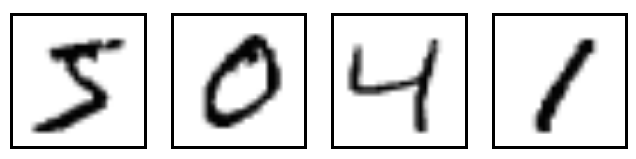
\includegraphics[width=0.7\textwidth]{Images/MNIST_images}
	\caption{Digit images from MNIST dataset}
	\label{fig:MNIST_images}
\end{figure}

Figure \ref{fig:MNIST_images} shows four examples of handwritten digit images from MNIST dataset, in order we have 5, 0, 4, 1.

\subsection{Usage in the machine learning}

As mentioned earlier, the MNIST dataset is widely used for training and testing neural networks, because it is a reference dataset in machine learning. During the years, lots of models in neural networks research were trained and tested on this dataset. Sometimes exciting results led to stale that neural networks achieved "near-human performance", but the first attempts obtained quite poor results: a linear classifier had a error rate from $12.0 \%$ to $7.6 \%$, which is really not satisfying for such a simple task.

Other solutions led to better results. Non-linear classifiers drastically reduced error rate to $3.3 \%$, but more appreciable results were obtained with 2-layers ($784-800-10$) neural networks, with an error rate of: $1.6 \%$, $0.7 \%$ with elastic distortion. Boosted stumps achieved an error rate of $0.87 \%$, support vector machines $0.56 \%$, K-nearest neighbors $0.52 \%$ and 6-layers deep neural network $0.35 \%$.

The best result have been achieved with \acsp{CNN}: different kinds of \acs{CNN} reached the lowest error rate, from $0.31 \%$ to $0.21 \%$. Although the problem is quite simple, it is clear that this kind of neural network is more powerful than others for this specific task.

\subsection{Technical informations about images}

The digits have been size-normalized and centered in a fixed-size image of $28x28$ pixels. The dataset includes labels for each image telling us which digit it is.

The original NIST dataset contained black and white, bilevel images. As a result of an anti-aliasing technique used in the normalization algorithms, images are now in greyscale. Digits were centered by computing the center of mass of the pixels and properly translating them.

Images are not in a standard image format, the data is stored in a very simple format designed for storing vectors and multidimensional matrices. Clearly labels values are from 0 to 9, while pixel values are from 0 to 255, 0 stands for white and can be found in the background, 255 is black and means foreground; pixels are organized row-wise. It is important to underline that in TensorFlow values 0 to 255 are normalized in the [0, 1] range.

\begin{figure}
	\centering
	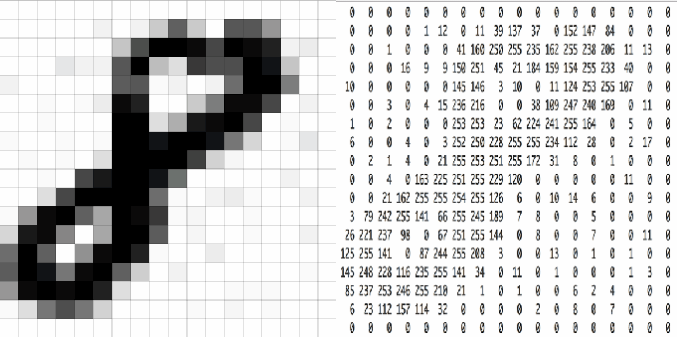
\includegraphics[width=0.9\textwidth]{Images/image_to_matrix}
	\caption{Example of translation from image to numeric matrix}
	\label{fig:image_to_matrix}
\end{figure}

Figure \ref{fig:image_to_matrix} shows an example of images storing format: each image can be translated into a numeric matrix, pixel by pixel, encoding pixel colors (white, black and grey levels) in the [0, 255] range.

More detailed informations about data format are not useful to read and compute the files in the dataset, but can be found on the \href{http://yann.lecun.com/exdb/mnist/}{dataset website}.

\section{Choosing the hyperparameters}

Now, let's focus on the simple model developed in tensorflow, starting from the hyperparameters choice.

Tuning the hyperparameters of the network is very delicate, it is a precision intervention which hopefully allows to improve both training and performances, but can also reduce them in the worst case. We will consider the following parameters: number of features to identify in every convolutional layer, filter size, stride size, number of input and output channels and padding of images.

\begin{description}
	
	\item[Number of features] This is one of the most important parameters to set, because here is specified how many features the network will try to identify. There is not a formula which allows us to find the perfect number of features based on the complexity of a task, but after several attempts with different values for this parameter we found a good solution for MNIST images. It can be concluded that a simple task, e.g. classifying $28x28$ grey scale images of digits, requires a small amount of filters to be learn (and consequently features to be identified): 8 in first convolutional layer, 16 in the second one. When we will analyze the results of the experiments, in Chapter \ref{ch:data_analysis}, with different values for this parameters, we will find that very good performances can be obtained with 2 and 4 features, too. More difficult task with bigger and higher quality images, would probably require tens or hundreds features. An opposite problem is a too high value, the result is that some filters became the same or very similar, so it could cause an increase in the complexity of the model without any benefit.

	\item[Patch size] The patch size allows us to adjust the size of the receptive field. Contrary to expectations, this parameter will not change from a convolutional and pooling layer to the next one, because while it is a fixed value, the image dimension is reduced, so the patch cover a greater area and allows the recognition of features, even more complex, in a bigger patch.  In our example with $28x28$ images a good patch size value is $5x5$. Obviously a bigger image would require an appropriately sized patch.
	
	\item[Stride size] According to the vanilla version proposed in the example, our stride value is 1. This value is combined with the padding in convolution and pooling in order to obtain an output of the same size of the input.
	
	\item[Input and output channels] These parameters can vary from a convolutional layer to another. In the first layer the input channel is linked to the colors of the input images, so in our example we have the value 1; the number of output channel depends on the number of features recognized in the layer. In deeper layers the input channel must correspond to the output channel of the previous layer, and the output channel to the features recognized in the layer.
	
	\item[Padding dimension and color] As described previously with the formula, we determined the zero padding dimension. It is very important because with the stride size value permit to keep stable dimensions of input and output layer after layer. It is important to notice that the color of the padding, i.e. white, corresponds to the color of the background of the MNIST images. It is a fluke, but what would happen if the padding color changed to black?

\end{description}

\section{The architectural level}

We introduced in Chapter \ref{ch:conv_nets} the different types of layers useful to build a \acs{CNN}, now we can analyze how they are combined in our TensorFlow model. This architecture was not modified, so it is exactly the one suggested in the TensorFlow example.

After the MNIST images are loaded, the TensorFlow session created and the variables initialized, we can start building the multilayer \acs{CNN}.

\subsection{Weights initialization}

First of all we need to define a matrix of weights, its dimensions depend on the parameter shape. At first weights are random values from a truncated normal distribution, the following lines of code shows their initialization.

\begin{lstlisting}
def weight_variable(shape):
  initial = tf.truncated_normal(shape, stddev=0.1)
  return tf.Variable(initial)
\end{lstlisting}

The parameter we passes to the function, shape, is a list containing the values of the different dimensions of the tensor.

We report also the bias initialization method in the following lines of code.

\begin{lstlisting}
def bias_variable(shape):
	initial = tf.constant(0.1, shape=shape)
	return tf.Variable(initial)
\end{lstlisting}

\subsection{First convolutional layer}

The following lines of code introduce the first block: a convolutional layer followed by a ReLU layer and a pooling layer. In the first two lines there are the weights and biases initializations; weights are random values from a truncated normal distribution, bias is a constant tensor. Then on the third line there are the convolution and the \acs{ReLU} operation, followed on the fourth line by the max pooling operation.

That kind of structure in the block we described is not the only solution, the different layers can be combined in different ways, e.g. we can add in this block a second convolutional layer instead of one before ReLU and max pooling.

\begin{lstlisting}
W_conv1 = weight_variable([5, 5, 1, features1])
b_conv1 = bias_variable([features1])
h_conv1 = tf.nn.relu(conv2d(x_image, W_conv1) + b_conv1)
h_pool1 = max_pool_2x2(h_conv1)
\end{lstlisting}

We can spend some words about the parameters of the function "weight\_variable": the two $5$ are the filter dimensions, while feature1 is the number of filters which corresponds to the number of feature the network will identify.

Figure \ref{fig:conv_layer} will help the reader to properly visualize the structure of this layer, from the patches on the image which we can see in the figure, connected to the feature maps in convolutional layer, to the feature maps connected to the max pooling layer.

\begin{figure}
	\caption{A detailed schema of a convolutional and pooling layer with detailed notations}
	\label{fig:conv_layer}
	\centering
	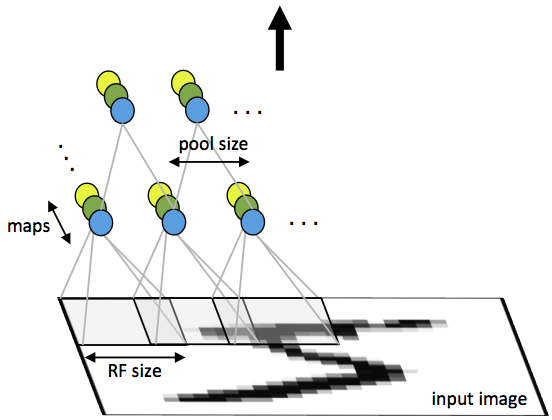
\includegraphics[width=1\textwidth]{Images/conv_layer}
\end{figure}

\subsection{Second convolutional layer}

Similarly to the previous subsection we can add a second block which has exactly the same structure of the first one: a convolutional layer with ReLU and pooling operations. The following code is equal to the previous, it does the same operations.

\begin{lstlisting}
W_conv2 = weight_variable([5, 5, features1, features2])
b_conv2 = bias_variable([features2])
h_conv2 = tf.nn.relu(conv2d(h_pool1, W_conv2) + b_conv2)
h_pool2 = max_pool_2x2(h_conv2)
\end{lstlisting}

The only difference between the two blocks we newly added is in the hyperparameters, in particular the number of features the network recognizes analyzing the images in input.

Any changes are possible: not only a single convolutional level can be added, but a whole block like the two we described right now. A more structured \acs{CNN} can be built with more complex task.

Even if we have so far tried to be clear and comprehensive describing this first part of the architecture in our basic model, we know it can be difficult to figure out the structure of all these levels. In order to help the reader, we provide in Figure \ref{fig:conv_layers} a visual description of the first two architectural blocks.

\begin{figure}
	\caption{A schema of the two convolutional and pooling layers with detailed notations}
	\label{fig:conv_layers}
	\centering
	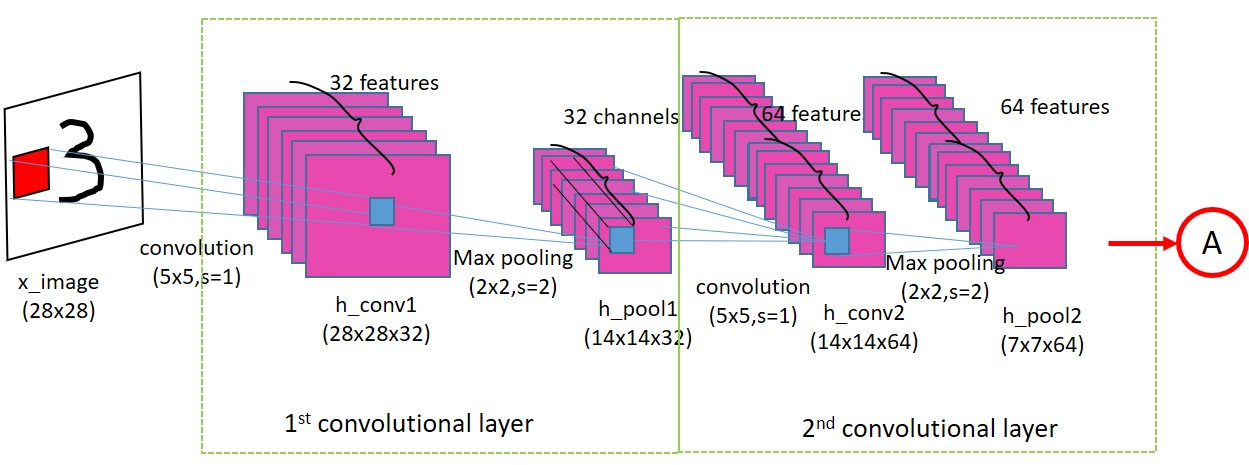
\includegraphics[width=1\textwidth]{Images/conv_layers}
\end{figure}

\subsection{Digression on the convolution and pooling functions}

We introduced two convolutional layers, but we only saw the call of mask functions, both for convolution and pooling. Now we can focus a little bit on these parts in the code, so below we will find the respective functions.

The first, as can suggest its name conv2d, is the function which performs the convolution operation. Its parameters are:

\begin{itemize}
	\item x, the 4d tensor, i.e. the images;
	\item W, The weights matrix;
	\item strides, as previously explained is 1;
	\item padding='SAME', output will have the same dimension of the input.
\end{itemize}

\begin{lstlisting}
def conv2d(x, W):
	return tf.nn.conv2d(x, W, strides=[1, 1, 1, 1], padding='SAME')
\end{lstlisting}

Similarly, in pooling function, max pooling exactly, we have again x, strides and padding, which we already explained.

\begin{lstlisting}
def max_pool_2x2(x):
	return tf.nn.max_pool(x, ksize=[1, 2, 2, 1], strides=[1, 2, 2, 1], padding='SAME')
\end{lstlisting}

\subsection{Densely connected layer}

The densely connected layer is the core of the classification process in our \acs{CNN}, it is implemented as matrix multiplication added to a bias offset. With that layer it is also possible to learn combinations of features.

We call the function weight\_variable to initialize the weights, the shape we define in the parameter is of dimension $7*7$ because we started from a $28x28$ image, in the first convolutional layer the max pooling reduced the dimensions to $14x14$, and similarly the second layer reduced it to $7x7$. And it is multiplied by the number of features identified in the second convolutional layer.

\begin{lstlisting}
W_fc1 = weight_variable([7 * 7 * features2, 1024])
b_fc1 = bias_variable([1024])
h_pool2_flat = tf.reshape(h_pool2, [-1, 7 * 7 * features2])
h_fc1 = tf.nn.relu(tf.matmul(h_pool2_flat, W_fc1) + b_fc1)
\end{lstlisting}

\subsection{Dropout layer}

In order to reduce overfitting we introduced a dropout layer, which is very important to better perform with new examples. The implementation of that operations is really simple: a random set of activations is set to zero, then the pruned nodes are reinitialized and reinserted into the network. The dropout layer is used only at training time, and not during testing.

In the following two lines of code we find the variable keep\_prob. This value specifies the probability that a node will be pruned or not.

\begin{lstlisting}
keep_prob = tf.placeholder(tf.float32)
h_fc1_drop = tf.nn.dropout(h_fc1, keep_prob)
\end{lstlisting}

As previously done, we provide another image, Figure \ref{fig:other_layers}, to help the reader figuring out the addiction of these new layers in the model architecture.

\begin{figure}
	\caption{A schema of the densely connected layer and dropout layer with detailed notations}
	\label{fig:other_layers}
	\centering
	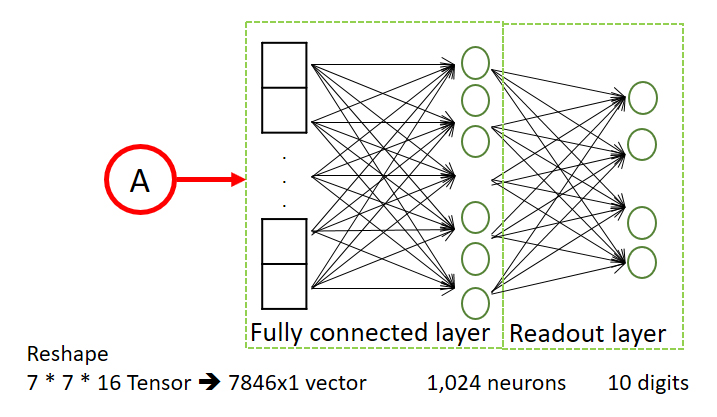
\includegraphics[width=1\textwidth]{Images/other_layers}
\end{figure}

\subsection{Loss (readout) layer}

The loss layer is the last one but also the core of regression model in our \acs{CNN}, here we find the implementation of regression model with the loss function: a multiplication of vectorized input images by the weight matrix, added to bias.

\begin{lstlisting}
W_fc2 = weight_variable([1024, 10])
b_fc2 = bias_variable([10])
y_conv = tf.nn.softmax(tf.matmul(h_fc1_drop, W_fc2) + b_fc2)
\end{lstlisting}

\section{Training, testing and evaluating the model}

\subsection{Training}

We have built our \acs{CNN} layer by layer, convolution by convolution and finally we defined the loss function. Our loss function is the cross entropy between the target and the softmax activation function applied to the model's prediction.

Now it is time to train that model and test its capabilities.

Train with TensorFlow allows to use automatic differentiation to find the gradient of the loss with respect to each of the variables. In the wide range of built-in optimization algorithms offered by TensorFlow we chose the Adam optimizer (Adaptive Moment optimizer) specifying in the parameter the learning rate. The optimizer adds new operations, which include ones to compute gradients, compute parameter update steps, and applied update steps to the parameters.

\begin{lstlisting}
cross_entropy = tf.reduce_mean(-tf.reduce_sum(y_ * tf.log(y_conv), reduction_indices=[1]))
train_step = tf.train.AdamOptimizer(1e-4).minimize(cross_entropy)
correct_prediction = tf.equal(tf.argmax(y_conv, 1), tf.argmax(y_, 1))
accuracy = tf.reduce_mean(tf.cast(correct_prediction, tf.float32))
\end{lstlisting}

Training the model can be therefore be accomplished repeatedly running the train\_step for a number of epochs.

\subsection{Testing and evaluating}

After a long training session, we want to evaluate performances of our network. It is possible with the following lines of code, where a percentage value of the accuracy is calculated.

\begin{lstlisting}
test_accuracy = accuracy.eval(feed_dict={x: mnist.test.images, y_: mnist.test.labels, keep_prob: 1.0})
\end{lstlisting}

Similarly we can evaluate the learning trend during the training epochs. It is one of the most important measurement we made during all the experiments we did with different parametrized \acs{CNN}.

\section{Modifications of the architecture}

Previously we talked about architectural interventions, classifying them as more structural modifications. We reinvented the wheel during the first tests, where we tried to change something in the layers structure adding convolutional levels. Disastrous results led us to the conclusions that in case of quite simple task, like digits classification, adding an excessive amount of layers ends up in unsatisfactory results. More precisely, adding only one layer to the structure we described above, the training curve did not converge. 

Just like the number of features should be assessed on the basis of task complexity, also the structure must be proportionate to it much more than hyperparameters.

Certainly tasks like facial recognition or high-defined images classification requires more complex structures, with more convolutional levels and much many features to be detected.

\section{GUI for real time testing}

In order to have new experiences with our \acs{CNN} a simple \acs{GUI} was implemented. It allows us to test our trained network with real data not coming from MNIST dataset.

The \acs{GUI} uses a pre-trained network which detects $16$ and $32$ features in first and second convolutional layer. Users can draw digits with the mouse in a small box. The input is then processed in order to make it similar to images from the MNIST dataset. In particular the digit is rescaled in order to fit a $28x28$ pixel grid. Color values are normalized from $0$ to $255$ range to $0$ to $1$. $1$ represents a black pixel, while $0$ a white one.

The processed image is then mapped to a $28x28$ numeric matrix which is the input for the neural network. The digit corresponding to the input matrix is finally shown to the user. Figures \ref{fig:GUI_5} and \ref{fig:GUI_8} show two examples of digit recognition using the \acs{GUI}, in the first one the model recognize and correctly classify a $5$, in the second a $8$.

\begin{figure}
	\caption{Example of the GUI and the recognition of handwritten digit 5}
	\label{fig:GUI_5}
	\centering
	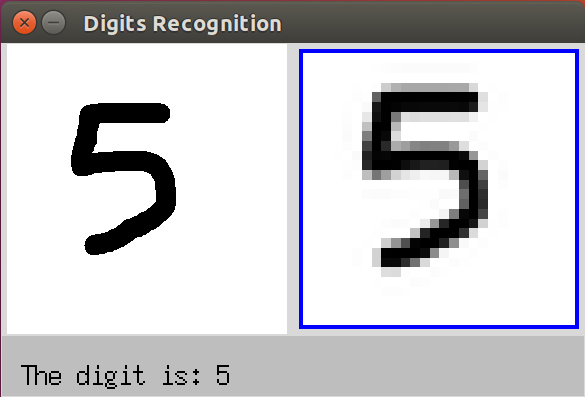
\includegraphics[width=0.8\textwidth]{Images/GUI_5}
\end{figure}

\begin{figure}
\caption{Example of the GUI and the recognition of handwritten digit 8}
\label{fig:GUI_8}
\centering
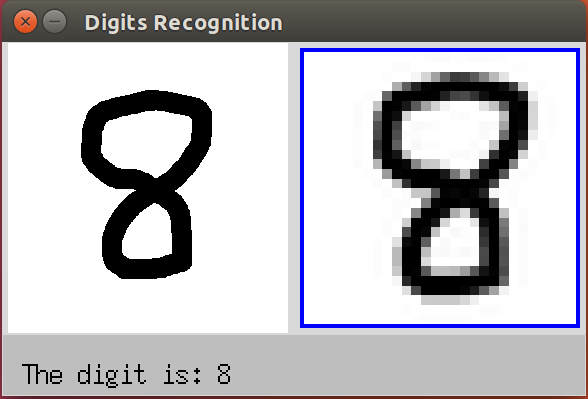
\includegraphics[width=0.8\textwidth]{Images/GUI_8}
\end{figure}

\section{Save and restore a TensorFlow model}

As we hint in Chapter \ref{ch:tensorflow_basics} at the end of the section about the variables, there is the possibility of save and restore the trained network, all the variables or only in part.

We used this functionality to train a network with $8$ features in the first convolutional layer and $16$ on the second, then reloading the saved variables we used the model to recognize handwritten digits with the GUI referred to in the previous section.